\newpage
\section{Optimal Reliability}

In the ISO 2394 norm on structural reliability \citep{iso2394} and the probabilistic model code by the joint committee on structural safety \citep{JCSS2000ProbabilisticDesign}, optimal reliability values are based on a cost function derived from the infinite renewal model of Rackwitz \citep{Rackwitz2000OptimizationVerification}, formulated as follows:
\begin{equation}
    \label{eqn:C_total}
    C_{total}(x) = C_{const}(x) + C_{const}(x) \frac{\omega}{\gamma} + (C_{const}(x) + C_H) \frac{P_f(x)}{\gamma}
\end{equation}
This quantifies the total lifetime monetary costs of a generic structure as a function of a decision parameter $x$ representing the structural design, with future costs discounted towards their net present value (NPV).
This consists of three components:

\begin{itemize}
    \item The initial construction costs $C_c = C_{const}(x)$, which are incurred once at the beginning of the lifetime of the structure. 
    \item The obsolescence costs $C_o = C_{const}(x)\frac{\omega}{\gamma}$, representing the structure being replaced with a yearly obsolescence rate $\omega$, incurring the construction costs again.
    These yearly costs are discounted using the yearly exponential discount rate $\gamma$ \citep{Green1996ExponentialTime}.
    \item The failure costs $C_f = (C_{const}(x) + C_H) \frac{P_f(x)}{\gamma}$, where $P_f(x)$ is the \emph{yearly} failure probability and $C_H$ are the additional damage costs incurred at failure, in addition to the construction costs for replacing the structure.
\end{itemize}

A linear function for $C_{const}(x)$ is often assumed, though this is not strictly necessary:
\begin{equation}
    \label{eqn:C_const_linear}
    C_{const}(x) = C_0 + C_1 x
\end{equation}
Where $C_0$ are costs independent of the decision variable, and $C_1$ represents the costs varying linearly with $x$.
Non-linear formulations could be used for $C_{const}(x)$ as well, as well as functions with multiple decision variables ($C_{const}(\mathbf{x})$), though these are rarely encountered in literature.
In general, $C_{const}(x)$ should be monotonically increasing. %($\frac{dC_{const}}{dx} \geq 0$ for all $x$).

The failure probability $P_f(x)$ is calculated through a reliability analysis, based on a limit state function $Z=g(x,\mathbf{R})$ and a set of random variables $\mathbf{R}$ with joint distribution $f_{\mathbf{R}}(\mathbf{r})$.
For a given value of the decision variable $x=x^*$, the failure probability is given by $P_f(x) = P[Z<0|x=x^*]=P[g(x^*,\mathbf{R})<0]$, together forming a probabilistic model of the structure.
For elementary limit state functions and probabilistic models \citep{Rackwitz2000OptimizationVerification}, an analytical expression of the failure probability may be available.
Otherwise, evaluating $P_f(x)$ requires a method such as FORM or Monte Carlo \citep{Ditlevsen2005StructuralMethods}.
% Generally, for increasing $x$, $P_f(x)$ should decrease with a decreasing slope ($\frac{dP_f}{dx} < 0$ and $\frac{d^2P_f}{dx^2} > 0$).

The definition of the decision variable $x$ is flexible.
In some literature, $x$ represents the ratio between the mean resistance of the structure $\mu_R$ and the mean load $\mu_S$ imposed on it ($x=\mu_R/\mu_S$) \citep{Rackwitz2000OptimizationVerification, Viljoen2012DerivingLQI}.
Less abstract quantities such as the section modulus of a beam are used as well \citep{Hingorani2023TowardsDesign}.

The optimal failure probability is found by minimising the cost function with respect to $x$, yielding the optimal value $x_{opt}$ and associated $P_{f,opt} = P_f(x_{opt})$ and $\beta_{opt}$:
\begin{equation}
    \begin{aligned}
        x_{opt} = \arg \min_{x} C_{total}(x)\\
    \end{aligned}
\end{equation}
Figure \ref{fig:generic_cost_Pf} visualises the optimisation problem.
Assuming the common linear formulation for $C_{const}$ is used, the parameter $C_1$ has a major influence on the optimal reliability: the larger it is, the more expensive additional reliability becomes, and the more the optimal failure probability is `pushed' upwards (for other formulations, any parameter influencing the positive slope of $C_{const}$ plays a similar role).
Similarly, the damage cost $C_H$ (which is generally much larger than $C_{const}(x)$ at the optimum) dominates the failure costs $C_f$ and `pulls' the optimal failure probability downwards.
This `push-pull' effect plays an important role in determining the optimal reliability of a structure, and becomes clear in the current norms.
ISO2394 defines three cost classes and three consequence classes by the relative magnitude of $C_1$ and $C_H$, respectively, and the combination of these classes determines the optimal reliability.
% In some literature \citep{Fischer2019OptimalDesign, Steenbergen2018TargetMaking}, the classes are defined by the ratio of $C_1$ and $C_H$ respectively to $C_0$ or $C_{const}$.
% A larger (relative) $C_H$ prescribes a larger $\beta_{opt}$ and smaller $P_{f,opt}$, while a larger $C_1$ causes the opposite.
Table \ref{tab:iso_table} presents these nine combinations, and thereby represents the current status quo for optimal reliability.



\begin{table}[h!]
    \caption{Conventional optimal failure probabilities, from \citep{iso2394}}
    \centering
    \begin{tabular}{c|lccc}
        Cost & &  \multicolumn{3}{c}{Consequence classes $C_H/C_0$}\\
        $C_1/C_0$ & & Minor & Moderate & Major\\ \hline
        
        Large & $\beta_{opt}$ &  3.1&  3.3& 3.7\\
          &$P_{f,opt}$& $10^{-3}$& $5 \cdot 10^{-4}$&$10^{-4}$\\ \hline
          
        Normal &$\beta_{opt}$ & 3.7 & 4.2 & 4.4\\
          &$P_{f,opt}$& $10^{-4}$& $10^{-5}$&$5\cdot10^{-6}$\\ \hline
        
        Small &$\beta_{opt}$ & 4.2 & 4.4 & 4.7\\
          &$P_{f,opt}$& $10^{-5}$& $5\cdot10^{-6}$&$10^{-6}$
    \end{tabular}    
    \label{tab:iso_table}
\end{table}


\begin{figure}[h]
    \centering
    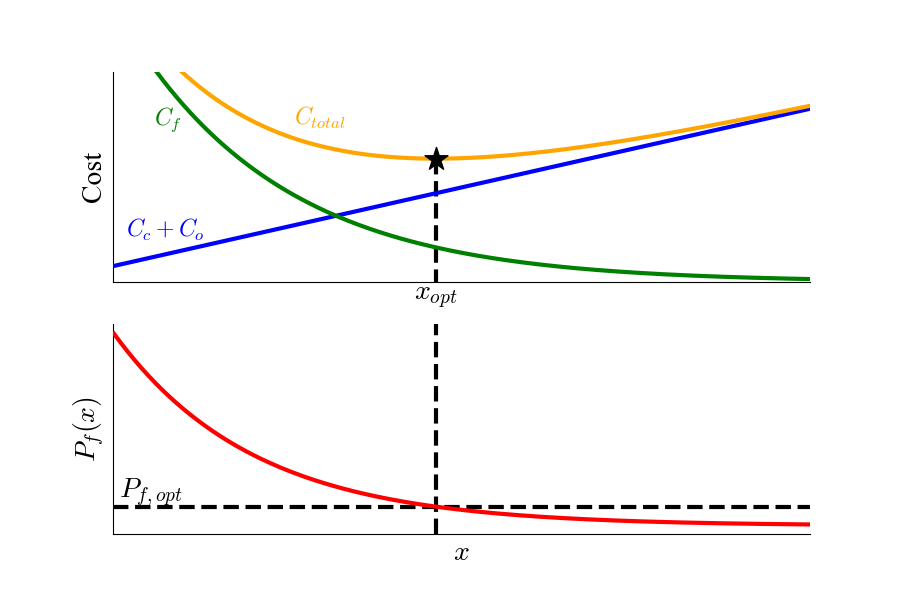
\includegraphics[width=0.95\linewidth]{Images/generic_cost_Pf.png}
    \caption{The optimisation underlying the current approach for determining optimal and acceptable reliabilities The blue line represents the `pushing' components of the cost function, and the green line the `pulling' failure costs}
    \label{fig:generic_cost_Pf}
\end{figure}





